\documentclass{article}

\usepackage[T1]{fontenc}
\usepackage[utf8]{inputenc}
\usepackage[frenchb]{babel}

\usepackage{hyperref}
\hypersetup{%
  colorlinks,%
  citecolor=black,%
  filecolor=black,%
  linkcolor=black,%
  urlcolor=black%
}

\usepackage{graphicx}
\graphicspath{{images/}}
\usepackage{subfig}
\usepackage{calc}

\usepackage{epigraph}

\usepackage{pgffor}
\usepackage{ifthen}
\usepackage{tikz}
\usetikzlibrary{matrix,fit,calc}

\usepackage{amsmath}
\usepackage[nottoc, notlof, notlot]{tocbibind}

\usepackage{rapport}

\author{Georges Dupéron}
\title{Langage de programmation}

\begin{document}

\maketitle
\tableofcontents
\newpage

\part{Objectif}

\section[Sujet]{Sujet: Etude d'un paradigme de programmation : les langages graphiques à Dataflow}
Il y a environ 20 ans, le langage et le système d'exploitation FORTH avaient été mis au point, avec pour but de créer un environnement
totalement personnalisé pour chaque utilisateur. La particularité de FORTH était qu'il ne possédait pas de mots-clés, ou instructions
figées, et que chaque utilisateur était en mesure de définir lui-même ses propres primitives, voire redéfinir ses primitives... à
l'infini.

L'échec de FORTH est venu, entre autres de la nécessité d'échanger des programmes entre utilisateurs, et des conflits dus à l'homonymie
(même nom, fonction différente) et à la synonymie (même fonction, noms différents). %Également, l'évolution des besoins et
Les fonctions n'étaient pas toujours documentées, ce qui fait qu'un même programmeur ne pouvait pas faire exécuter, à un intervalle de
temps relativement court, 2 fois le même programme...

Pour autant, le côté adaptatif et souple de FORTH aurait été largement plébiscité s'il n'y avait eu cette difficulté. Une manière de
contourner ce genre de conflit, dû à une représentation symbolique textuelle trop fortement contrainte par la syntaxe, est de se pencher
vers une programmation qui privilégie les flux de données sur les actions à réaliser, et vers des bases graphiques plutôt que textuelles,
laissant donc à chaque utilisateur la liberté de définir ses actions, et préservant en revanche les flux.

L'idée de ce projet est de proposer une première architecture de compilateur ou d'interpréteur de premier niveau pour illustrer ce
paradigme, et tenter d'en évaluer les propriétés. Ce projet nécessite un excellent niveau en programmation et un goût prononcé pour
l'écriture de compilateurs.

\section{But du projet}
Le but de ce projet sera donc dans un premier temps de définir un langage de programmation visuel utilisant le paradigme du
dataflow\footnote{\url{http://en.wikipedia.org/wiki/Dataflow}}, et n'ayant pas de primitives fixes. Dans un second temps, nous
implémenterons un EDI\footnote{Environnement de Développement Intégré} permettant de créer des programmes dans ce langage, et de les
interpréter.

\part{Définition du langage}

\section{Étude de l'existant}

\subsection{FORTH}\footnote{Les bibliothèques universitaires de Montpellier n'ont aucun ouvrage concernant FORTH. Il faudrait peut-être suggérer quelques achats aux bibliothécaires.}
Le langage FORTH est basé sur le principe de l'expansion de macros~: lorsqu'on «appelle» une macro, elle s'expanse, ses sous-macros
s'expansent, et ainsi de suite, jusqu'à ce que des macros de bas niveau lisent des valeurs sur la pile (pop), et en écrivent d'autres à la
place.

Mon expérience personnelle, lorsque j'ai essayé par le passé d'implémenter des algorithmes un peu complexes en \TeX (le langage sur
lequel est construit \LaTeX), m'a montré que cette approche a un défaut fondamental~: il est impossible de délimiter le rayon d'action d'une
macro. Étant donné qu'elle travaille sur la pile (ou dans le cas de \TeX, sur les jetons qui suivent l'appel de macro), et qu'elle peut
enlever ou ajouter autant d'éléments qu'elle veut sur la pile, il y a un risque assez grand pour qu'une macro dont on ne connaît pas bien le
fonctionnement soit mal utilisée, et abîme la portion de pile qui appartient à d'autres macros.

Vu que les macros peuvent être imbriquées autant qu'on veut, il est possible qu'une macro située très bas dans l'arbre fasse ce genre
d'erreur. Le débogage nécessite alors de parcourir tout l'arbre d'appels de macros à la recherche de l'erreur.

Une représentation graphique permet d'indiquer explicitement quelles sont les données fournies à une fonction ou une macro, et il devient
alors possible de mettre en place des mécanismes de contrôle de l'utilisation de la pile, au moins pour le débogage. Sans cette approche, il
n'y a aucun moyen de savoir quels sont les données passées en paramètre et quelles données doivent rester sur la pile, du point de vue de la
macro appellante.

Dans le cas de FORTH, il n'y a pas de primitives dans le langage. Cela signifie que si on regarde récursivement le code des macros, il n'y a
pas un moment où on va tomber sur une macro qui n'a pas de définition, mais est implémentée par le compilateur ou l'interpréteur (définition
dans un autre langage, et probablement inaccessible pour peu qu'on n'ait pas le code source du compilateur). À la place, aux feuilles de
l'arbre d'expansion des macros, on trouvera des instructions du langage machine.

Ce comportement est fortement souhaitable de la part d'un langage généraliste, du point de vue éducatif~: les curieux peuvent farfouiller
jusqu'aux racines du langage et ainsi comprendre comment fonctionne les programmes, à tous les niveaux. Certains programmeurs pensent que
c'est important de comprendre en profondeur comment fonctionne la machine et les programmes qui l'utilisent\cite{coders-at-work}.

Cela confère aussi au langage une grande portabilité~: FORTH a été porté sur plus d'une vingtaine de processeurs\cite{forth-history}. En définissant un ensemble
de fonctions de haut niveau que chaque implémentation doit fournir, on peut s'assurer qu'un programme fonctionnant sur une implémentation du
langage fonctionnera aussi sur une autre.

\subsection{Dataflow}

Le paradigme du dataflow\cite{vanroy-paradigms} (flux de données) est connu des concepteurs de langages de programmation depuis longtemps. Il a été utilisé avec
succès dans certains domaines, principalement des domaines intéressant les non-programmeurs.

\subsubsection{Graphisme}

Le logiciel Quartz Composer sous MacOS permet la création d'images vectorielles animées et interactives sous MacOS de manière graphique~: On
applique des filtres graphiques, représentés par des boîtes, aux résultats d'autres filtres, en connectant les boîtes entre elles. Dans
World Machine, ces filtres sont des actions physiques (érosion, soulèvement) et permettent de générer des cartes de hauteur (heightmaps),
qui sont utilisées pour modéliser des terrains en 3D.

\subsubsection{Musique}

L'interface de certains logiciels de musique s'inspirent de l'architecture des synthétiseurs modulaires\cite{modular-synth} (ces grosses
boîtes avec pleins de prises jack qu'on relie avec des câbles : chaque prise jack est une entrée ou une sortie d'un module, les câbles sont
les connexions). Un des premiers synthétiseurs virtuels, Max/MSP, utilisait cette analogie. D'autres logiciels similaires lui ont succédé :
PureData (qui est aussi un langage de programmation généraliste), Alsa Modular Synth,~\dots

% http://recherche.ircam.fr/equipes/repmus/RMPapers/CMJ98/

\subsubsection{Mesures scientifiques}

LabView permet aux scientifiques de procéder à des traitements sur les signaux et les données acquises depuis un ordinateur, grâce à un
langage de programmation graphique utilisant le paradigme du dataflow.

\begin{figure}[ht] 
  \setbox1=\hbox{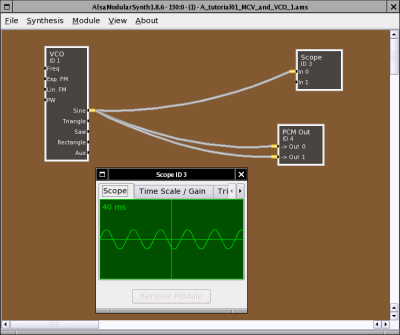
\includegraphics[width=5cm]{alsa-modular-synth}}% The smaller image 
  \setbox2=\hbox{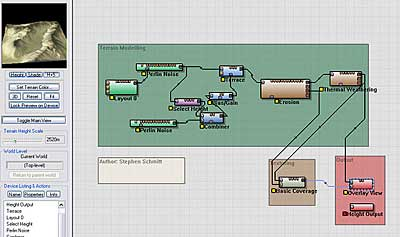
\includegraphics[width=5cm]{world-machine}}% The larger image 
  {\,}
  \hfill 
  \begin{minipage}{5cm}
    \centering
    % http://cafcom.free.fr/ams/ams1.png
    \raisebox{0.5\ht2-0.5\ht1}{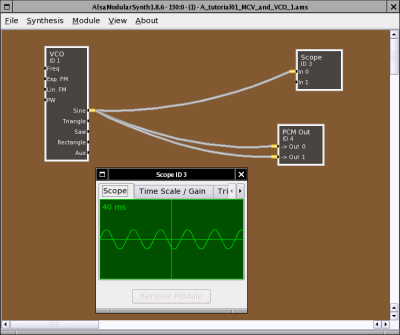
\includegraphics[width=5cm]{alsa-modular-synth}}
  \end{minipage}
  \hfill
  \begin{minipage}{5cm}
    \centering
    % http://www.world-machine.com/images/ui1.jpg
    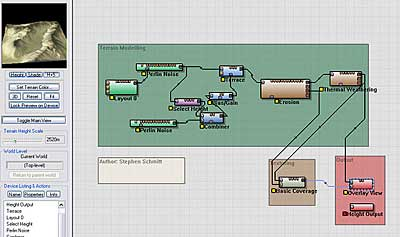
\includegraphics[width=5cm]{world-machine}
  \end{minipage}
  \hfill
  {\,}
  
  %%%%%%%%%%
  
  {\,}
  \hfill 
  \begin{minipage}{5cm}
    \centering
    \caption{Alsa Modular Synth\cite{alsa-modular-synth}}
    \label{fig:alsa-modular-synth}
  \end{minipage}
  \hfill
  \begin{minipage}{5cm}
    \centering
    \caption{World Machine\cite{world-machine}}
    \label{fig:world-machine}
  \end{minipage}
  \hfill
  {\,} 
  
  %%%%%%%%%%%%%%%%%%%%%%%%%%%%%%%%%%%%%%%%%%%%%%%%%%
  
  \setbox1=\hbox{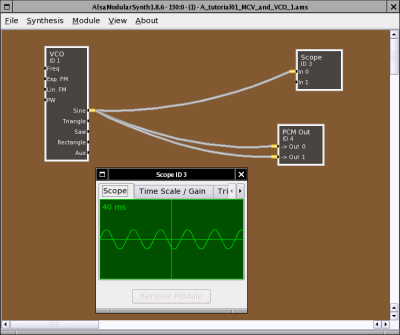
\includegraphics[width=5cm]{alsa-modular-synth}}% The smaller image 
  \setbox2=\hbox{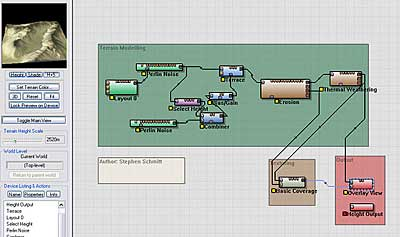
\includegraphics[width=5cm]{world-machine}}% The larger image 
  {\,}
  \hfill 
  \begin{minipage}{5cm}
    \centering
    % http://upload.wikimedia.org/wikipedia/en/thumb/b/bc/QuartzComposerSnowLeopard.png/800px-QuartzComposerSnowLeopard.png
    \raisebox{0.5\ht2-0.5\ht1}{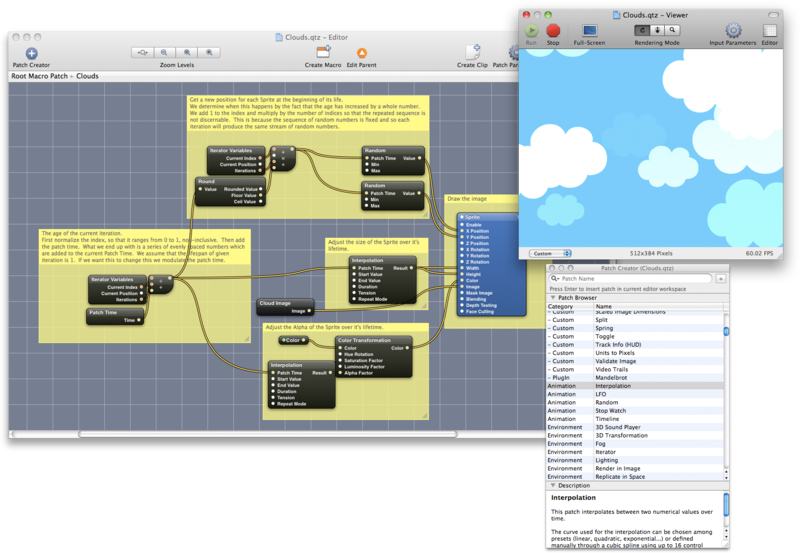
\includegraphics[width=5cm]{quartz-composer}}
  \end{minipage}
  \hfill
  \begin{minipage}{5cm}
    \centering
    % http://zone.ni.com/cms/images/devzone/tut/binary_tree2.png
    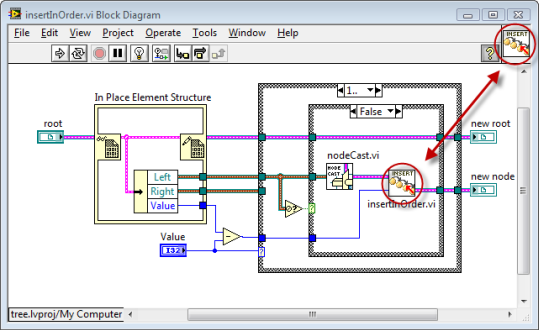
\includegraphics[width=5cm]{labview}
  \end{minipage}
  \hfill
  {\,}
  
  %%%%%%%%%%
  
  {\,}
  \hfill 
  \begin{minipage}{5cm}
    \centering
    \caption{Quartz Composer\cite{quartz-composer}}
    \label{fig:quartz-composer}
  \end{minipage}
  \hfill
  \begin{minipage}{5cm}
    \centering
    \caption{LabView\cite{labview}}
  \end{minipage}
  \hfill
  {\,} 
  \caption{Captues d'écrans de quelques langages de programmation utilisant le paradigme du dataflow.}
  \label{fig:screenshots}
\end{figure}

\subsubsection{Traitement de signaux}

Force est de constater que tous les exemples cités ci-dessus sont des cas particuliers de traitement de signal (image, son, signaux
provenant d'appareils de mesure). Le paradigme du dataflow devrait être tout aussi efficace pour construire des programmes conventionnels~:
les signaux d'entrée sont les évènements provoqués par l'utilisateur (clic de souris, appui sur le clavier), ceux de sortie sont les retours
(écran, haut-parleurs, \dots).

\subsection{langages visuels}

\subsubsection[Acceptation par les programmeurs]{Acceptation des langages visuels par les programmeurs}
Les langages visuels n'ont eu que peu de succès auprès de la communauté des programmeurs, et les raisons de ce rejet méritent d'être
étudiées\footnote{Peut-être que c'est simplement que les langages textuels, c'est pour les programmeurs avec du poil sur le torse, et les
  langages graphiques sont pour les mauviettes…}.

Récemment, un chercheur a mis en place un sondage auprès des programmeurs qui devrait à terme permettre de savoir quels langages
correspondent le mieux à quelles affirmations, selon les programmeurs\cite{the-right-tool}. Ces affirmations sont du type «Ce langage est
facile à utiliser» ou «Ce langage a une bonne communauté». Les affirmations qui obtiennent les moins bons scores pour un langage donné
indiquent en général les défauts de ce langage. J'ai donc contacté l'auteur de ce sondage pour lui demander d'ajouter des langages de
programmation visuels pendant que le sondage est encore ouvert, afin de pouvoir étudier par la suite ces résultats.

\subsubsection{Historique}
On a toutefois de noubreux cas d'utilisation de représentations visuelles dans la programmation~: Les langages suivant le paradigme du
dataflow, dont nous avons parlé ci-dessus, mais aussi l'utilisation d'un formalisme graphique pour la représentation principale des
diagrammes UML\footnote{Il existe aussi une représentation textuelle d'UML\cite{htun-spec}}. Les organigrammes de programmation (control
flow diagram) sont aussi utilisés depuis longtemps.

D'autres représentations visuelles sont utilisées dans certains systèmes. La figure \ref{fig:lisp-class-graph} montre un graphe d'héritage
des classes en Lisp avec l'environnement McCLIM. On trouve aussi des graphes d'appels de fonctions, qui relient deux fonctions si l'une
appelle (ou peut appeler) l'autre.

\begin{figure}[h!]
  \centering
  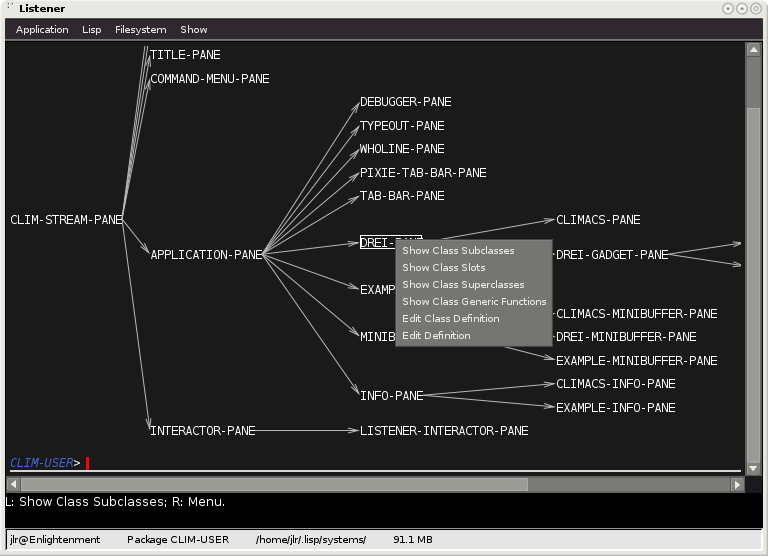
\includegraphics[width=10cm]{lisp-class-graph}
  \caption{Graphe d'héritage des classes en Lisp avec McCLIM}
  % On http://mcclim.cliki.net/Screenshot : http://jlr.freeshell.org/data/mcclim/screenshots/2007-03-27-listener-dark-classgraph-context-menu.png
  % http://boinkor.net/lisp/porn/clim-debugger.png
\label{fig:lisp-class-graph}
\end{figure}

\subsection{Langages spécifiques à un domaine}
\label{sec:dsl}

Il est fréquent que des programmeurs créent des «langages spécifiques à un domaine» (DSL, Domain Specific Language) pour répondre au besoin
d'exprimer facilement des instructions et notions très fortement liées à un certain domaine, sans être encombrés par la syntaxe rigide, le
vocabulaire limité et le manque d'expressivité de leur langage habituel. Les fichiers de configuration sont en général écrits dans un DSL
par exemple. Mais les DSL ont de grosses limitations : bien qu'ils soient adaptés à l'expression d'idées dans ce domaine, ces langages ne
possèdent pas l'expressivité nécessaire à des opérations plus complexes~: souvent, ces DSL ne sont complets au sens de Turing et n'ont pas
accès aux bibliothèques de fonctions des autres langages.

C'est pour ces raisons que les DSL sont de plus en plus laissés un peu de côté~: La configuration de GRUB 2 est toujours dans un DSL, mais
elle est générée dynamiquement par des scripts shell\cite{config-grub}, la configuration du gestionnaire de fenêtres awesome est écrite en
Lua\cite{config-awesome}, beaucoup de logiciels utilisent python comme langage de script, plutôt que de créer un langage de script
spécifique à l'application.

D'un autre côté, le problème des langages de programmation généralistes est qu'ils permettent d'augmenter le vocabulaire disponible, par
l'ajout de fonctions et la création de variables, mais ils ne permettent pas de modifier la grammaire utilisé (la structure du code). En
réalité, de nombreux langages permettent cela par le biais de macros, mais cette approche est assez limitée~: l'écriture de macros est en
général fastidieuse -- beaucoup plus difficile que l'écriture de fonctions -- et l'utilisation de macros est néanmoins soumise à un grand
nombre de contraintes syntaxiques du langage hôte (parenthèses, accolades, \dots). De plus le système de macros de certains langages, comme
le C, n'a pas la puissance d'un vrai langage : pas de récursivité des macros, pas de structures conditionnelles à l'intérieur d'une macro.

Il y a donc des avantages dans les deux approches, mais aucune ne permet de satisfaire complètement les besoins de facilité d'expression et
de puissance du langage. Nous proposons une solution alternative~: permettre l'écriture d'un programme sous n'importe quelle forme visuelle
(grammaire libre), dans un langage graphique orienté dataflow. Nous imposons quelques contraintes, afin de garder une certaine cohérence~:
\begin{itemize}
\item Les sous-programmes sont représentés par des éléments graphiques (blocs) ;
\item Les paramètres d'entrées de ces sous-programmes sont des entités visuelles qu'on peut connecter entre elles (ports) ;
\item Les valeurs de ces paramètres sont fournies à travers des liens qui relient les ports ;
\end{itemize}
Ces règles laissent toutefois une très grande liberté, les blocs peuvent être rectangulaires, ronds ou de n'importe quelle forme. Ils
pourraient par exemple afficher les calculs mathémathiques qu'ils contiennent non pas sous l'apparence d'instructions mais d'une formule
mathémathique. On peut aussi faire en sorte que dans un outil de conception d'interfaces utilisateur, les composants graphiques (fenêtre,
bouton, etc.) ne soient pas de simples images, mais \emph{soient} les fonctions ou objets correspondants. Dans le logiciel LabView, les
«blocs» peuvent revêtir différentes apparences.
% TODO screenshot en pgf pour la formule mathémathique.

Il est même possible que certains blocs aient une apparence invisible. Par exemple les opérations de conversion de types (cast) pourraient
être masquées, et ne s'afficher que sur le lien entre la source du transtypage et sa destination.

Avec ces règles, les ports n'ont pas besoin d'être affichés en permanence. Ils peuvent par exemple être dans une boîte de dialogue de
configuration dui apparaît lorsqu'on double-clique sur le bloc correspondant (World Machine utilise cette approche, et laisse aussi les
ports visibles en mode «réduit»).

Les liens peuvent être annotés, regroupés en bus, etc. Comme on peut l'imaginer, avec un minimum d'effort de cohérence, ces libertés sont
susceptibles de rendre les programmes plus lisibles (non-affichage des éléments qui ne sont pas importants à la comprhéension du programme)
et plus faciles à écrire (les instructions (blocs) spécialisées ont une interface d'utilisation adaptée).

\subsection{Environnement de développement intégré}

{
  \setlength{\epigraphwidth}{0.85\linewidth}
  \renewcommand{\textflush}{justify}
  \renewcommand{\epigraphflush}{center}
  \epigraph{
    Clearly good design is as important for visual languages as for textual ones. Furthermore, the effectiveness of a visual language indeed
    any precise language for specifying structures, depends to a large extent on the quality of the editor, browser, interpreter, debugger and
    other tools supplied by the language implementation
  }{Christopher C. Risley and Trevor J. Smedley \cite{the-editor-is-as-important-as-the-language}}
}

Les environnements de développement intégré jouent un rôle crucial pour les langages de programmation visuels. En effet, sans la possibilité
de construire un programme par une séquence (obscure) de caractères, la convivialité du langage est directement liée aux outils que propose
l'EDI. Ces EDI n'ont en général que peu en commun avec les ceux destinés aux langages textuels, et se présentent plus comme des logiciels de
dessin vectoriel que comme des éditeurs de texte.

Certaines questions sont récurrentes dans la conception d'EDI pour des langages visuels. Une des plus importante est la gestion de l'espace
à l'écran~: les primitives graphiques sont décorées de bordures, et d'autres éléments visuels, qui occupent beaucoup d'espace à l'écran,
réduisant ainsi la quantité d'informations affichées. Ce problème est plus communément connu sous le nom de «Deutsch
Limit»\cite{deutsch-limit}~:
\begin{quotation}
  Well, this is all fine and well, but the problem with visual programming languages is that you can’t have more than 50 visual primitives
  on the screen at the same time. How are you going to write an operating system?
\end{quotation}

Cependant, dans le cas d'un affichage textuel, le cerveau humain n'est pas capable d'ingurgiter en temps réel toute l'information à
l'écran\footnote{Sur mon écran, on peut loger plus de 60 lignes de texte verticalement, et ce sur 2 colonnes. Allez donc analyser 120 lignes
  de C d'un seul coup.}. L'affichage sous forme graphique permet au contraire de clarifier et de nettoyer les informations à l'écran, on
peut donc supposer que le cerveau est capable d'analyser plus rapidement du «code» graphique que son équivalent textuel (un dessin vaut
mille mots, dit-on).

De plus les programmeurs passent beaucoup de temps à chercher tel ou tel morceau de code ou fonction. L'EDI Code Bubbles\cite{code-bubbles}
apporte une solution à ce problème pour les langages textuels, en fournissant une interface dans laquelle le programmeur manipule un gand
nombre de fragments de code assez court, et a la possibilité d'en ouvrir facilement de nouveaux de manière contextuelle (ouvrir la
définition de cette fonction, ouvrir la documentation de celle-là). Nous avons repris ce principe pour les langages visuels~: Dans la
définition d'un bloc, il est possible d'ouvrir sur place ou à côté les définitions des sous-blocs.

Une autre solution consiste à utiliser une interface «fish-eye»~: les objets au centre de l'écran ont une taille normale, et sont de plus en
plus petits à mesure qu'ils approchent du bord. Une variante est l'interface «zoom», utilisée notamment dans certains jeux
vidéos\cite{mutant-storm} pour permettre au joueur de focaliser son attention sur les ennemis les plus proches, ou bien avoir une vue
d'ensemble, et dans le logiciel de prises de notes Project Cecily\cite{project-cecily}.

Plusieurs recherches ont été menées concernant l'utilisation de l'espace à l'écran par les langages visuels, une bibliographie référencant
plusieurs papiers sur ce sujet est disponible à \cite{biblio-vpl-a-screen-real-estate}.


\subsection[Manque d'expressivité]{Manque d'expressivité des langages de programmation existants}

L'utilisation fréquente de «design patterns» ou partons de conception dans les langages de programmation existants peut être considérée
comme un indicateur de défauts dans ces langages\cite{design-patterns-failure}~: s'il y a besoin d'utiliser le design pattern $x$, c'est
que le langage ne permet pas d'utiliser les concepts vehiculés par $x$ de manière plus élégante, c'est donc un manque d'expressivité sur ce
point. En général, la manière la plus élégante d'utiliser un concept, c'est quand il est de «première classe».

La solution que nous proposons pour un autre problème d'expressivité, celui des Langages Spécifiques à un Domaine (Section \ref{sec:dsl},
page \pageref{sec:dsl}), qui était de permettre aux blocs de revêtir n'importe quelle apparence, est aussi une solution aux problèmes
soulignés par les Design Patterns. En effet, pour peu que le langage propose de l'introspection et que les éléments de base du langage
soient (réellement) de première classe, à savoir les blocs, les ports et les connexions, il est possible de transformer un grand nombre de
concepts en concepts de (pseudo-)première classe.

Par exemple, si l'on souhaite implémenter le concept des singletons, on rajoutera par introspection à chaque bloc utilisant ce concept un
faux port d'entrée qui représentera directement le singleton. Ou bien on encapsulera tous les blocs représentant des variables qui doivent
être uniques, avec une structure qui s'assurera que tout accès à ces blocs se fera sur une unique instance.

\subsection{Réutilisabilité}

\subsubsection{Programmation par composants}

Le paradigme du dataflow partage de nombreux points communs avec le paradigme de la programmation orientée composants. Cette approche vise à
augmenter la ré-utilisabilité du code en le structurant sous forme de composants qui communiquent entre eux. Dans le paradigme du dataflow,
les composants sont clairement visibles~: ce sont les blocs, et ils communiquent entre eux à travers leurs ports, par le biais de
connexions.

\subsubsection{Commandes Unix}

Ce principe de composants isolés communiquant au travers d'interfaces pré-définies se retrouve aussi dans l'architecture Unix. Un des
principes de la philosophie unix est «Do one thing, and do it well», ainsi sous Unix, plein de petis programmes différents font chacun une
action bien précise, simple. Des actions plus complexes sont réalisées en connectant la sortie de certains programmes à l'entrée d'autres,
en général avec un «pipe» (tuyau).

Ce principe a même été poussé jusqu'à faire un navigateur modulaire, suivant la philosophie Unix, dont la partie chargée d'afficher les
pages web est complètement dissociée de la partie qui gère les autres fonctionnalités (historique, boutons de navigation, \dots).

Cependant, cette approche est très limitée, car le seul type de données que des programmes peuvent échanger au travers de pipes ou de
sockets, c'est un flux d'octets augmenté d'un marqueur de fin (EOF). Il n'y a pas de communication hors-bande, pas de structuration des
données. Cela pose des problèmes d'encapsulation (au sens des protocoles de communication~: comment envoyer plusieurs flux en parallèle?),
d'échappement, et généralement de sérialisation des données -- alors qu'on transfère des données d'un programme à l'autre, sur le même
système.

Le paradigme du dataflow résoud ces problèmes en permettant de faire transiter à travers les connexions entre blocs des flux typés, plutôt
que de simples octets. De plus, chaque bloc possède plusieurs ports de sortie, ce qui permet de sélectionner la donnée voulue. Sous Unix,
pour récupérer la date de modification d'un fichier, il faut découper la sortie de la commande \texttt{ls -l} avec d'autres outils, comme
\texttt{cut}. En dataflow, il suffit de faire une connexion uniquement avec le port de sortie intitulé «taille du fichier».

%\begin{itemize}
%\item Héritage partiel (cf. tiddlywiki)
%\end{itemize}

%\begin{figure}[htbp]
%  \centering
%  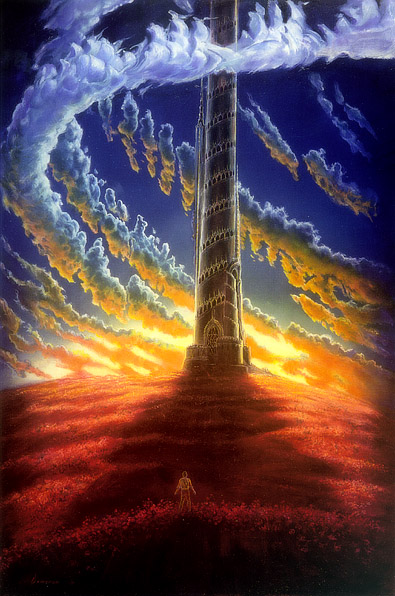
\includegraphics[height=7cm]{dark-tower-of-meta-levels}
%  \caption{Aziz faces the Dark Tower of Meta-levels}%\footnote{http://www.phyast.pitt.edu/~micheles/scheme/scheme22.html}
%  % On http://www.phyast.pitt.edu/~micheles/scheme/scheme22.html
%\label{fig:dark-tower-meta-levels}
%\end{figure}

\subsubsection{Conflits de nommage}
Les conflits de nommage sont une grosse source de souci dans les langages de programmation textuels conventionnels. Certains utilisent des
espaces de nommage pour réduire les risques de conflits, d'autres utilisent les clôtures pour limiter la portée des noms (c'est ce qui est
couramment utilisé en JavaScript, par exemple).

Nous proposons une approche différente, qui consiste à stocker avec chaque fonction définie un identifiant unique, comme si le code était
stocké dans une base de données. Les appels de fonction font alors référence (de manière cachée) à l'identifiant unique, et non pas au «nom
usuel» de la fonction. Cela rend le langage insensible aux conflits de nommage, et robuste aux changements des noms de variables ou de
fonction. D'autres personnes ont proposé de stocker du code Java dans une base de données\cite{scid}.

\section{Formalisation du langage}

%Dans cette section, nous allons essayer de trouver quelle est la nature, l'essence d'un programme, de manière à 

\subsection{Programme en dataflow}

Examinons un programme simple exprimé dans le paradigme du dataflow~:

\begin{figure}[h]
  \centering
  \begin{tikzpicture}
    \bloc[t]{+1/a+b}{ab}{c}
    \tikzset{+2/.style={below of=+1,matrix anchor=north}}
    \bloc[t]{+2/a+b}{ab}{c}
% \tikzset{b2/.style={right of=b1-out-d,matrix anchor=b2-in-x.center}}
%    \bloc[t]{b2/\frac{x\times y}{z}}{{x}{y}{z}}{{t}}
    
    \tikzset{e1/.style={left of=+1-in-a,matrix anchor=e1-out-val.center,input-bloc}}
    \bloc[t]{e1/e_1}{}{{val/}}
    \draw (e1-out-val) -- (+1-in-a);
    
    \tikzset{e3/.style={left of=+2-in-b,matrix anchor=e3-out-val.center,input-bloc}}
    \bloc[t]{e3/e_3}{}{{val/}}
    \draw (e3-out-val) -- (+2-in-b);
    
    \tikzset{e2/.style={at=($ .5*(e1-out-val) + .5*(e3-out-val) $),matrix anchor=e2-out-val.center,input-bloc}}
    \bloc[t]{e2/e_2}{}{{val/}}
    
    \node[coordinate] (between-+1-+2) at ($ .5*(+1-in-b) + .5*(+2-in-a) $) {};
    \node[coordinate] (connect-e2-+1-+2) at ($ .5*(between-+1-+2) + .5*(e2-out-val) $) {};
    
    \draw (e2-out-val) -- (connect-e2-+1-+2);
    \draw (connect-e2-+1-+2) |- (+1-in-b);
    \draw (connect-e2-+1-+2) |- (+2-in-a);
    
    
    \shorthandoff{:}
    \draw[->] (+1-out-c) -- ++(1,0) node[coordinate,label=above:\tiny$e_1+e_2$] {};
    \draw[->] (+2-out-c) -- ++(1,0) node[coordinate,label=below:\tiny$e_2+e_3$] {};
    \shorthandon{:}
  \end{tikzpicture}
  \caption{Un programme simple en dataflow.}
\label{fig:simple-dataflow}
\end{figure}

Ce programme a trois entrées ($e_1$, $e_2$, $e_3$), et deux sorties ($e_1+e_2$ et $e_2+e_3$).

\subsection{Caractéristiques du programme}
La question à se poser maintenant est ~:
\begin{figure}[h!]
  \centering
  Qu'est-ce qui définit ce programme ?
\end{figure}

Ou, comme le disait un des collègues de Joe~Armstrong~\cite{what-are-the-inputs}\nocite{coders-at-work}~:

\begin{figure}[h!]
  \centering
  \begin{quotation}
    «~A program is a black box. It has inputs and it has outputs. And there is a functional relationship between the inputs and the outputs. What are the inputs to your problem ? What are the outputs to your problem ? What is the functional relationship between the two ?~»
  \end{quotation}
\end{figure}

Ce programme est constitué
\begin{itemize}
\item d'entrées,
\item de sorties,
\item d'un graphe étiqueté exprimant la relation entre les sorties et les entrées grâce à des fonctions ($+$) qu'on suppose déjà définies,
\item d'une sémantique d'évaluation, qui donne une signification au graphe,
\item d'une représentation graphique,
\item Et pour l'exécuter pour de bon, il faut une machine réelle vers laquelle on peut compiler le programme (ou un interpréteur fonctionnant sur cette machine).
\end{itemize}

\subsection{Généralisation}
Si on généralise ce résultat, on peut dire qu'un programme est défini par une structure de données abstraite (on n'a pas besoin de connaître la représentation en mémoire de cette structure), qui peut contenir des entrées, des sorties, un arbre (ou graphe) syntaxique, etc. Cette structure peut être représentée sous forme d'un programme dont l'entrée est la désignation d'une partie de la structure que l'on souhite accéder, et dont la sortie est la partie en question.

La représentation graphique ou textuelle du programme peut être assurée par un autre programme.

Sa sémantique d'évaluation peut être définie par une machine abstraite, dont les (méta-)entrées sont le programme, ainsi que des entrées pour le programme, et dont les (méta-)sorties sont les sorties que le programme devrait avoir. Tiens ? Entrées, sorties, une relation fonctionnelle (les sorties sont celles du programme pour ses entrées), \dots\ Eh oui, notre machine abstraite, c'est-à-dire notre sémantique d'évaluation est bel et bien un programme elle aussi.

De même, la machine réelle vers laquelle on éspère pouvoir compiler le programme, peut être modélisée par un programme. Pendant que nous y sommes, rien ne justifie la présence de la machine réelle, car la machine abstraite pourrait très bien être la même que celle qui exécute le programme. C'est le cas par exemple si notre langage est le code machine d'un certain processeur : L'octet 0x12345678 a pour signification «diviser l'accumulateur par 2», c'est une définition de la sémantique du langage, et à la fois une définition de la machine qui exécute le programme.

La machine abstraite n'a donc pas besoin d'être si abstraite que ça, et pourrait être n'importe quelle machine, et il pourrait même y avoir plusieurs machines qui spécifient la sémantique du langage (de manière redondante, pour avoir le choix, et pour que ces définitions se vérifient mutuellement).

Et, pour continuer sur cette voie, il peut aussi y avoir plusieurs représentations syntaxiques (textuelle, avec ou sans coloration, graphique, \dots).

On a donc les équations suivantes dans le cas simple (une seule machine, une seule représentation) :

\begin{align}
  \text{Programme} &= \left\lbrace
      \begin{array}{rl}
          &\text{Type de données abstrait (ADT)}\\
        + &\text{Machine abstraite (sémantique)}\\
        + &\text{Représentation}
      \end{array}
      \right\rbrace\\
  \text{Programme} &= \text{Programme} + \mathrm{Programme} + \mathrm{Programme}\\
  \text{Programme} &= 3 \times \text{Programme}
\end{align}

\subsection{Base}

Nous voilà bien avancés\dots\ Un programme est un programme. C'est donc une définition récursive. Et toute définition récursive doit avoir une base, et des règles pour générer de nouveaux éléments. Nous venons de définir les règles, cherchons les bases possibles~:
\begin{itemize}
\item Machine de Turing
\item Lambda-calcul
\item Langage mathémathique
\end{itemize}

Le lambda-calcul et la machine de Turing sont
équivalents\cite{lambda-calculus-wikipedia}$\vphantom{X}^{,}$\footnote{Bien qu'ils ne
  semblent pas être totalement équivalents\cite{lambda-turing-equivalence}~: \quote{However, [Lambda Calculus] is not a model of computation for we
    cannot calculate an upper bound on resource consumption of its reduction steps without resorting to another model of computation, such
    as [Turing Machines] (according to Yuri Gurevich).}},
% http://conal.net/blog/posts/can-functional-programming-be-liberated-from-the-von-neumann-paradigm/#comment-35342
% A lambda calculus program does describe a computable function. However, LC is not a model of computation for we cannot calculate an upper
% bound on resource consumption of its reduction steps without resorting to another model of computation, such as TMs (according to Yuri
% Gurevich). But, models of computation don’t end there, either.
par contre le langage mathémathique permet d'exprimer des fonctions non-calculables, des ensembles infinis, et tout un tas de choses
obscures. Comme nos machines physiques actuelles sont une version bâtarde des machines de Turing (qui n'ont pas de limite sur la quantité de
mémoire disponible, contrairement aux nôtres), il semble sage de laisser de côté le langage mathémathique (pour l'instant, lorsque le
langage aura gagné en maturité, peut-être qu'il sera temps de l'ajouter).

L'équivalence $\lambda$-calcul vs. Turing nous laisse le choix pour l'implémentation de notre première machine à partir de laquelle les autres seront définies, directement ou indirectement. Explorons donc la suite du problème avant de prendre une décision. À terme, le meilleur sera probablement d'implémenter les deux, comme base, et de les définir mutuellement l'une à partir de l'autre, pour avoir une vérification.

\subsection{Graphe}
Du point de vue de notre langage, on peut dire qu'un programme est un graphe dont les noeuds sont étiquetés (les noms ou identifiants des blocs), et dont les arcs sont étiquetés à chaque extrémité (les noms des deux ports auxquels le lien est connecté). Les programmes sont donc des graphes généralisés.

% TODO !!!!!!!!!!!!
% Schéma PGF

% Preuve de complétude de Turing : un graphe = des noeuds connectés par des arcs, un noeud = l'arc NULL ou qqch du genre. <=> $\lambda(\lambda(\dots))$.


\part{Implémentation}
%Pour l'implémentation, nous nous limiterons à un sous-ensemble purement fonctionnel du langage défini dans les sections précédentes.

\section{Spécification fonctionnelle}



\appendix

\nocite{*}
\bibliographystyle{unsrt}
\bibliography{biblio}

%%%%%%%%%%

\long\def\commentaire#1{}

\commentaire{
\part{Annexes}
%\section{Notes}
%\subsection{notes}
%\begin{itemize}
%\item gruntnetwork.com
%\item La thèse sur la programmation par l'exemple
%\item vidéo alan kay
%\end{itemize}

%\section{Étude de l'existant}
%Preuves

% Taxonomie (vltax.pdf): étudier l'utilité des différentes catégories.


\subsection{Notes pour la suite\dots}

Cette section est à supprimer

% Suite
%Partir d'un plus haut niveau pour se faciliter la tâche : une VM simple en JahvaScript
%Définir une api de base (?), c'est une machine virtuelle sur laquelle s'exécuteront les programmes
%  - Structures de données
%  - Dataflow


%%%
%X Définir le langage grunt par rapport à une VM simple (et cette VM à partir d'une machine de Turing)
%  Prendre un programme grunt, et l'expanser au maximum (FORTH). Descendre jusqu'au niveau des transistors ou au moins des bascules.

Nous allons prendre un programme en dataflow, et le déconstruire le plus possible, afin de voir quelles sont les «primitives» sémantiques nécessaires à notre langage. Bien que FORTH n'ait pas à proprement parler de primitives, il a lui aussi une sémantique (chaque mot est expansé en la suite de mots le définissant, jusqu'à arriver au code machine).
  

Il faut définir un bloc eager-evaluation, qui prend en paramètre un graphe, et
\begin{itemize}
\item Soit le réécrit (compilation)
\item Soit l'évalue (interprétation)
\end{itemize}
Dans le cas où on compile, on aura une "instruction" call-bloc

call-bloc prend en paramètre des fonctions permettant de calculer ses paramètres, ainsi que les paramètres eux-mêmes.
\begin{itemize}
\item En évaluation paresseuse, on n'évalue les paramètres que s'ils sont nécessaires.
\item En évaluation «eager», on évalue les paramètres au début de l'appel du bloc, et on stocke leur valeur pour une future utilisation (ou non).
\item Pour une macro, on stocke juste les paramètres eux-mêmes (avec leur fonction d'évaluation, s'il y en a une).
\end{itemize}

TODO première ligne de \section{Formalisation du langage}
}

\end{document}
